\section{Sharpening in the spatial domain}

\subsection{Blur difference image}
\begin{figure}[ht]
\centering
	\subfigure[Base Cameraman image]{
	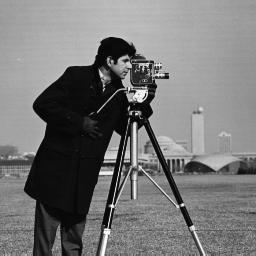
\includegraphics[width=0.45\linewidth]{question4/1_camBase}
	}
	\subfigure[Original image - Blurred image]{
	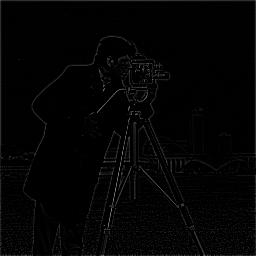
\includegraphics[width=0.45\linewidth]{question4/1_cam_highBoost}
	}
\end{figure}



\subsubsection{What does the subtracted image look like? What frequency components from the original image are preserved in the subtracted image? Why?}
The subtracted image looks an outline of the original image (i.e. edges are preserved). The Gaussian blurred image attenuates the high frequency components, and leaves the low frequency components relatively untouched. When subtracting this blurred image from the original image, only the high frequency components of the original image will remain.

\clearpage
\subsection{High-boosting filtering}
\begin{figure}[ht]
\centering
	\subfigure[High-boosted image, A=1.0]{
	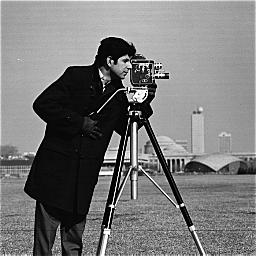
\includegraphics[width=0.45\linewidth]{question4/2_cam_highBoost_10}
	}
\end{figure}

\subsubsection{What does the resulting image look like? How does it differ from the original image? Explain why it appears this way}
The resulting image from adding the subtracted image back to the original image is a sharper image. This process is referred to a high-boost filtering. This image appears sharper as the high frequency components in the original image have been doubled by adding the high frequency components of the original image back to the image.

\clearpage
\subsection{High-boosting coefficients less than unity}

\begin{figure}[ht]
\centering
	\subfigure[High-boosted image, A=1.0]{
	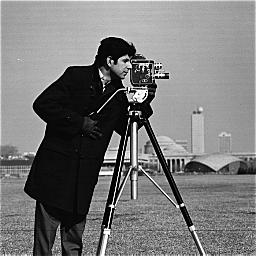
\includegraphics[width=0.45\linewidth]{question4/2_cam_highBoost_10}
	}
	\subfigure[High-boosted image, A=0.5]{
	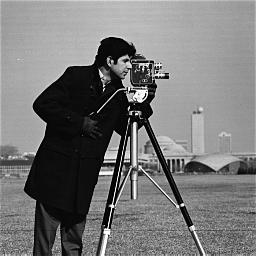
\includegraphics[width=0.45\linewidth]{question4/3_cam_highBoost_05}
	}
\end{figure}
\subsubsection{Compare the results produced by adding the subtracted image to the original image and that produced by adding half of the subtracted image to the original image. How does it differ? Explain why it appears this way}
The edges are less prominent in the image with half the subtracted image added. This is because the high frequency components are accentuated less. However, the high frequency noise in the background of the image (the sky) is also less prominent.

\clearpage
\subsection{High-boosting coefficients greater than unity}
\begin{figure}[ht]
\centering
	\subfigure[High-boosted image, A=1.5]{
	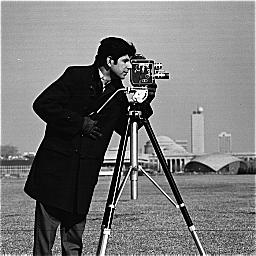
\includegraphics[width=0.45\linewidth]{question4/3_cam_highBoost_15}
	}
	\subfigure[High-boosted image, A=4.0]{
	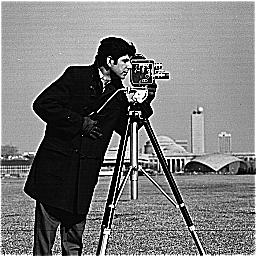
\includegraphics[width=0.45\linewidth]{question4/3_cam_highBoost_40}
	}
\end{figure}

\subsubsection{What does multiplying the subtracted image by a factor less than one accomplish? What about greater than one}

When multiplying it by a factor less than one, edges are not as sharp, but high frequency noise is also less magnified. When multiplying the high-boost coefficient by a value greater than one, the image can be over-sharpened, and ringing artifacts can occur, as well as loss of any gentle variations in high frequency regions (in the A=4.0 image, the grass looks awful).
